\chapter{Random Networks} \label{Appendix_A}

\begin{comment}
We did some simulations with python to prove the claims we have done before.\footnote{The python scripts can be found in the GitHub page of the author at the link: \url{https://github.com/ShqemzaMatteo/Master_thesis}} 

To begin, we analyze a toy model: diffusion over a ring network with the same probability to go left and right; therefore the Adjacency matrix and the Laplacian of the Network are both symmetric and the balance detail holds. The simulation start with the particle in a fixed probability distribution; next, it applies the stochastic dynamics and it takes note of the path that the particle has chosen. The simulation repeat the process 500 times and, then, we compute the probability distribution for each node for each update. In this way we have found experimentally the evolution of the probability distribution. 
After that, we can calculate the Shannon entropy entropy $S(t) = \sum_i p_i(t)\ln p_i(t)$, where $p_i(t)$ indicates the probability that the particle is in the node $i$ at time $t$, and the Von Neumann entropy $\sum_\lambda p_\lambda(t) \ln p_\lambda(t)$, where $p_\lambda(t)$ indicates the probability that the particle is in the mode $\lambda$ at time $t$.
Furthermore, we compute the Von Neumann entropy of the network following equation \ref{Von_Neumann_Entropy} with the density matrix \ref{density_matrix_evolution}. 

\smallskip

The different entropies are plotted in figure \ref{fig:pure_states} for pure state: in the left the initial distribution is a delta centered in a fixed node; in the right it begins with a uniform distribution over the nodes. It can be seen that the experimental Von Neumann entropy has the same trend respect to the theoretical one and, despite the Shannon one that increases, they are constant at zero value. The perturbation can be consider as thermal fluctuation. 

\begin{figure}[ht!]
    \centering
    \begin{subfigure}[t]{.49\textwidth}
        \centering
        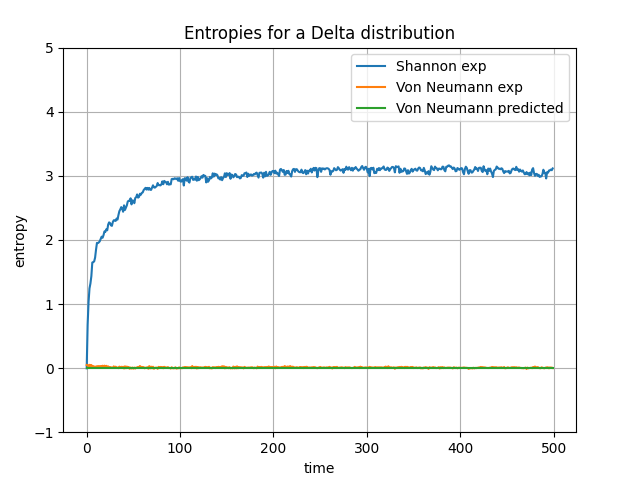
\includegraphics[width=\linewidth]{image/Delta.png}
        \label{fig:delta}
    \end{subfigure}
    \hfill
    \begin{subfigure}[t]{.49\textwidth}
        \centering
        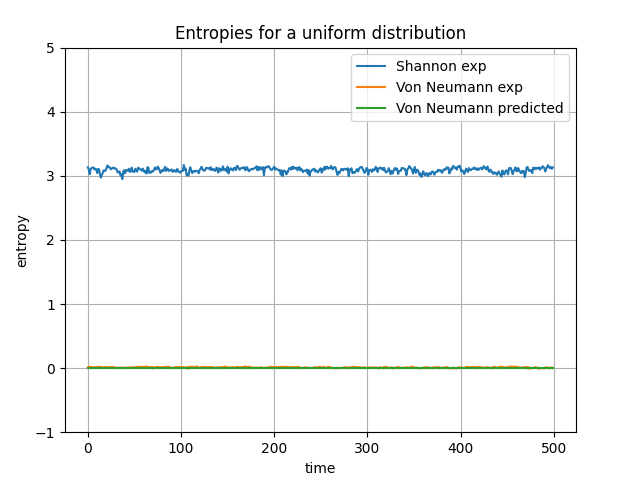
\includegraphics[width=\linewidth]{image/Uniform.png}
        \label{fig:uniform}
    \end{subfigure}
    \caption{Plot of different entropies in function of time with different initial density matrix: on the left, the network begins with a delta distribution peaked in one node; on the right, the network starts on a uniform distribution over the nodes. In blue the Shannon entropy from the experimental data, in orange the Von Neumann entropy from experimental data, in green the Von Neumann entropy as \ref{Von_Neumann_Entropy}. It can be seen that the theoretical and experimental Von Neumann entropy are close and both have a decreasing trend.}
    \label{fig:pure_states}
\end{figure}
\begin{figure}[ht!]
    \centering
    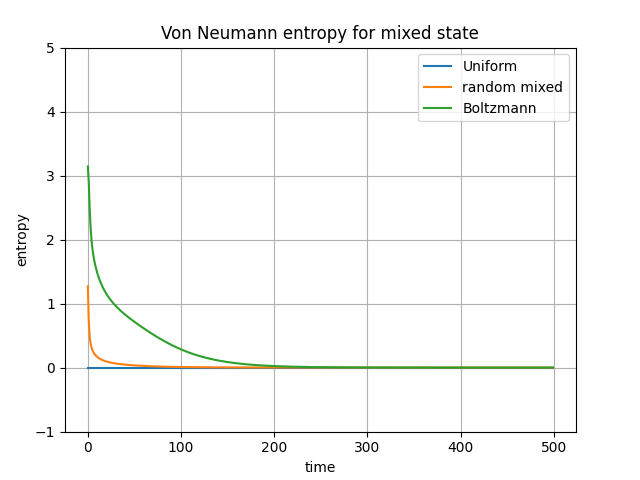
\includegraphics[width=0.65\linewidth]{image/mixed_state.png}
    \caption{Plot of Von Neumann entropy in function of time of a network with mixed density matrix: in green, $\hat\rho(0) = e^{-\beta \hat L}$; in orange, the density state is a mixed of 100 randomly chosen pure state with random weight; in blu, the uniform distribution over the nodes.}
    \label{fig:mixed_state}
\end{figure}


\break
The simulation for mixed state are plotted in figure \ref{fig:mixed_state}, but, because of the vague meaning of mixed state over network, they show only the plot for the theoretical ones. In the picture there are plotted several network with different starting point: uniform distribution (which is a pure state); a mixed state form by the sum of $100$ randomly generated pure state with random weight; the state of equilibrium at temperature $T$. All the different mixed states show a exponential decreasing trend.

After checking the right behavior of the simulations, we analyze the trend of the maximal entropy state $\hat \rho(t) = \exp\left(-\frac{\beta}{2}\hat L\right)$ increasing $\beta$. In figure \ref{fig:ER-BA-WS}, it is shown the plot of the Von Neumann entropy for this state varying beta for a ring graph, for Erd\H{o}s-Rényi (E-R) random graph \cite{erdos-renyi1960} with connectivity probability $0.7$ and for a Barab\'abi-Albert (B-A) scale-free graph \cite{Barabasi_Albert_1999} with parameter $m=3$, and the Watts-Strogatz (W-S) small world graph \cite{Watts-Strogatz_1998} with parameter $m=3$ and rewiring probability $0.2$.
All graphs have a decreasing trend, but E-R and B-A have a faster decreasing than the other two
\begin{figure}[ht!]
    \centering
    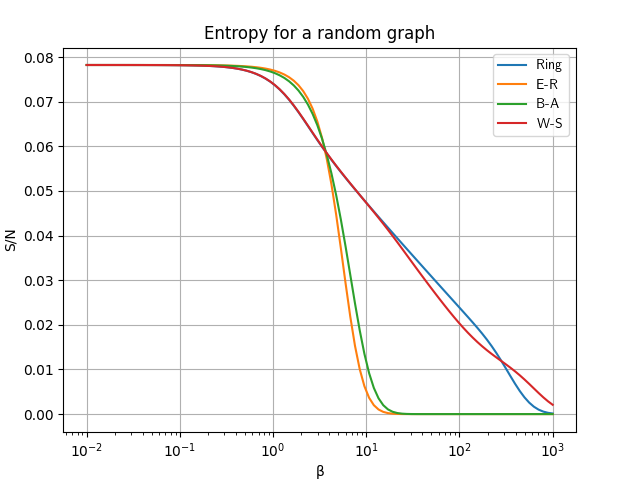
\includegraphics[width=0.65\linewidth]{image/random_graph.png}
    \caption{Plot of Von Neumann entropy in function of $\beta$ for a maximal entropy state over a ring graph, in blue, over a Erd\H{o}s-Rényi (E-R) random graph with connectivity probability $0.7$, in orange, for a Barab\'abi-Albert (B-A) scale-free graph with parameter $m=3$, in green, and for a Watts-Strogatz (W-S) small world graph with parameter $m=3$ and rewire probability 0.2, in red.}
    \label{fig:ER-BA-WS_2}
\end{figure}
\end{comment}

During the dissertation, we have introduce various type of random graph: in this appendix we do a brief introduction to each of them.

\section{Erd\H{o}s-Rényi random graph}

The Erd\H{o}s-Rényi random Graph $G(N,M)$ \cite{erdos-renyi1960}, where $N$ and $M$ are respectively the number of nodes and links, is one of the first attempt to generate a random network. The network is build choosing at random M links from all the possible ones. Usually, is used the contraction proposed by Gilbert $G(N,p)$ \cite{gilbert} , where $p$ is the probability that two distinct node are connected. The two formulations converge in the thermodynamic limit $N \rightarrow \infty$ and they are interchangeable.
This type of random graph has peculiar properties as the distribution of the degree of the nodes $P(k)$  is binomial
\begin{equation}
    P(k) = \binom{n-1}{k}p^k(1-p)^{n-1-k}
\end{equation} 
and, also, if $p > \frac{1}{N}$ then is almost sure that the network presents a giant component.
In this work we use the second approach. In figure \ref{E-R_example} it is shown two example of E-R random graph, one below and one above the giant component threshold.

\begin{figure}[ht!]
    \centering
    \begin{subfigure}[t]{0.49\textwidth}
        \centering
        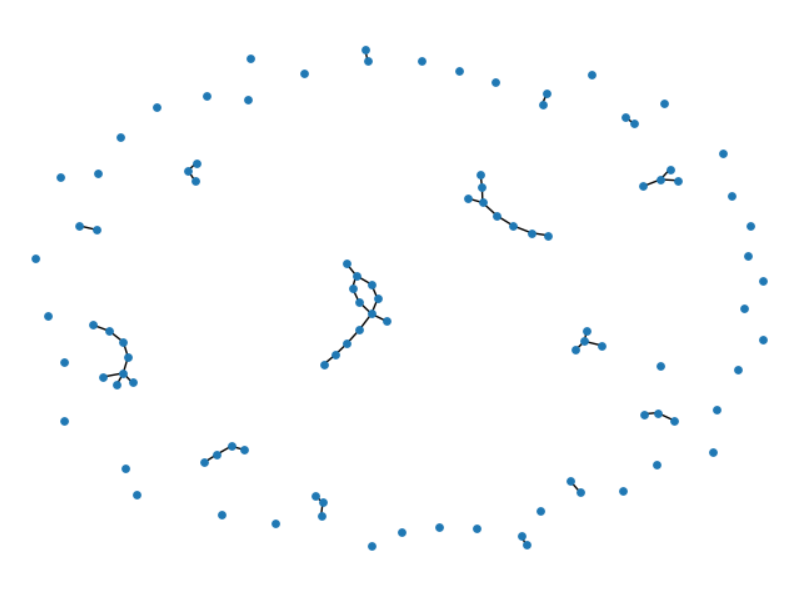
\includegraphics[width=\linewidth]{image/E_R_N100_p0,01.png}
    \end{subfigure}
    \hfill
    \begin{subfigure}[t]{0.49\textwidth}
        \centering
        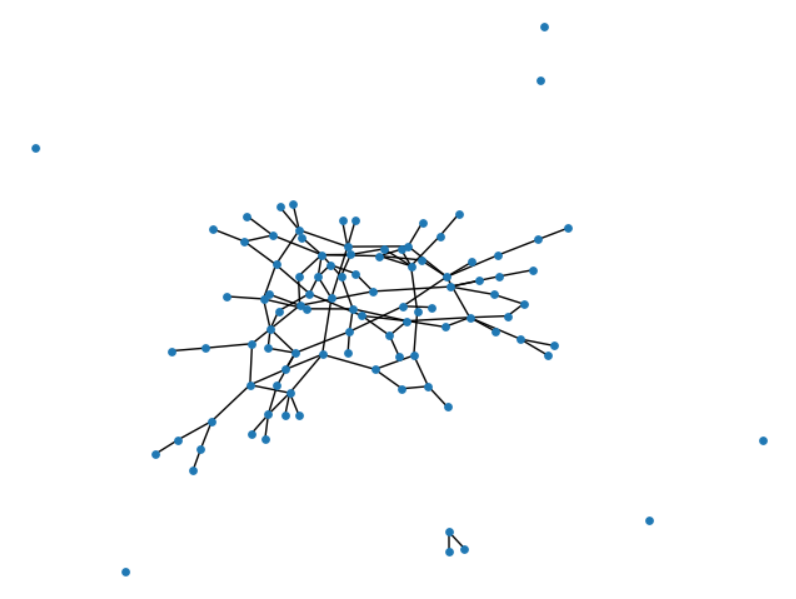
\includegraphics[width=\linewidth]{image/E_R_N100_p0,02.png}
    \end{subfigure}
    \caption{Two example of Erd\H{o}s-Rényi random graphs: on the left, it has 100 nodes and $p = 0.01$; on the right, it has 100 nodes and $p = 0.02$. Overcoming the threshold $p > 0.01$ can be seen the formation of the giant component.}
    \label{E-R_example}
\end{figure}
%the algorithm is define as below :
%\begin{enumerate}
 %   \item we identify the graph by its adjacency matrix;
 %   \item For each possible link, we generate a random number, if it is less than $p$ the respective entry in the adjacency matrix  is 1 otherwise 0.
%\end{enumerate}

However, the E-R algorithm do not produces network similar to the real ones found in nature, they tend to be more clustered and to have hubs (nodes with very high degree). To simulate this properties new algorithms have been proposed, like the Barab\'abi-Albert scale-free network and the Watts-Strogatz small world network.

\section{Barab\'abi-Albert scale-free network}
Barab\'abi and Albert proposed a scale-free Network $G(N, m)$ \cite{Barabasi_Albert_1999} that mimics the behavior of real graph like the Internet. This type of graph shows some preferential nodes which have a degree order of magnitude higher that the average and present a power law as degree distribution.
The model works by preferential attachment, where new nodes are more likely to connect to nodes that already have a higher degree. 

The algorithm is define below:
\begin{enumerate}
    \item It is initialized a complete graph of $m_0 > m$ node, usually $m_0 = m+1$;
    \item The other nodes are connected to this graph: for each new node, it is connected to $m$ nodes with probability $p_i = \frac{k_i}{\sum_i k_i}$, where $k_i$ is the degree of the $i$ node.
\end{enumerate}
In figure \ref{B-A_example} it is shown two example of B-A networks.

\begin{figure}[ht!]
    \centering
    \begin{subfigure}[t]{0.49\textwidth}
        \centering
        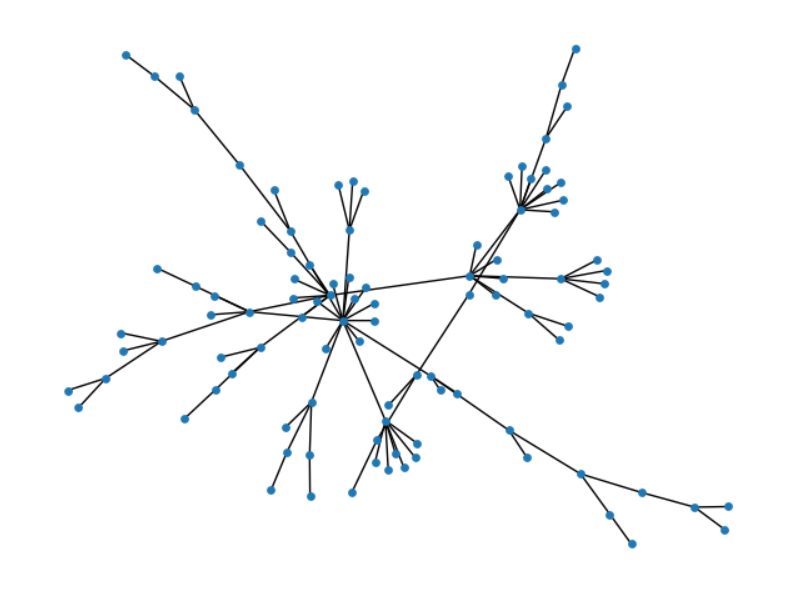
\includegraphics[width=\linewidth]{image/B_A_N100_m1.png}
    \end{subfigure}
    \hfill
    \begin{subfigure}[t]{0.49\textwidth}
        \centering
        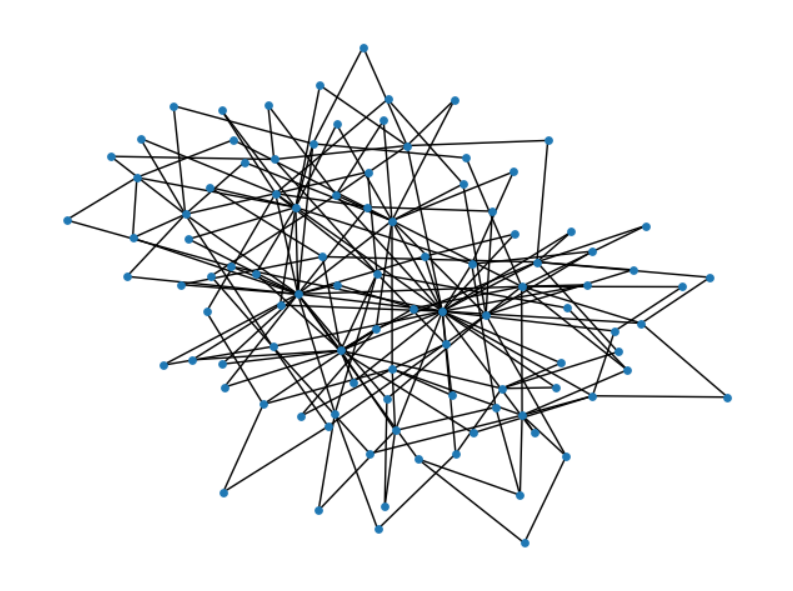
\includegraphics[width=\linewidth]{image/B_A_N100_m2.png}
    \end{subfigure}
    \caption{Two example of Barab\'abi-Albert scale-free networks: on the left, it has 100 nodes and $m=1$; on the right, it has 100 nodes and $m=2$.}
    \label{B-A_example}
\end{figure}

\section{Watts-Strogatz small world network}

The Watts-Strogatz small world network $G(N, K, p)$ \cite{Watts-Strogatz_1998}, where $N$ is the number of nodes, $K$ is the average degree (it must be even) and $p$ is the rewiring probability, is a model that exhibit high clustering and short average path lengths. The degree distribution is a power law and the network is homogeneous, all nodes have similar degree.

The algorithm is shown below:
\begin{enumerate}
    \item It is created a ring network with $N$ nodes where each node is connect to the $K/2$ nearest neighbors for each side;
    \item For each edge with probability $p$, the link is removed and another one to node chosen uniformly at random is created, the new link must be a not existing one.
\end{enumerate}

In figure \ref{W-S_example} it is shown two example of W-S networks.

\begin{figure}[ht!]
    \centering
    \begin{subfigure}[t]{0.49\textwidth}
        \centering
        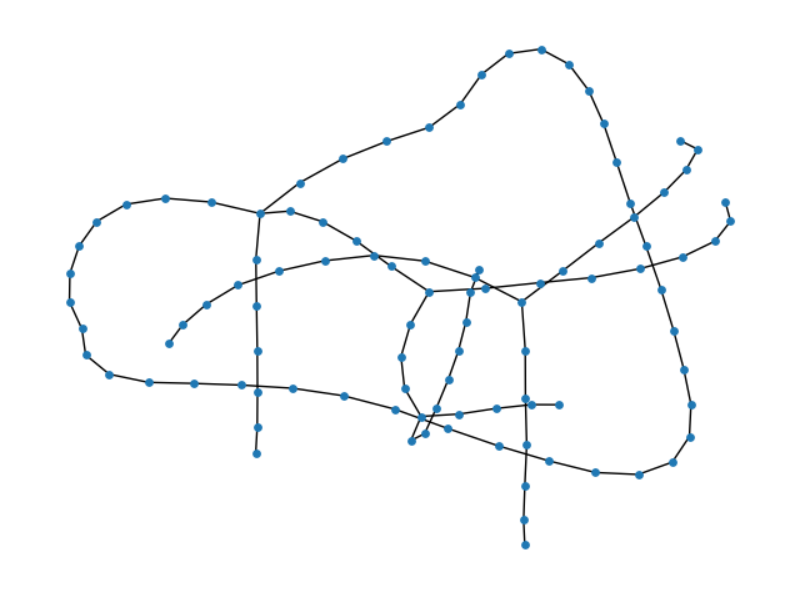
\includegraphics[width=\linewidth]{image/W_S_N100_K2_p0,1.png}
    \end{subfigure}
    \hfill
    \begin{subfigure}[t]{0.49\textwidth}
        \centering
        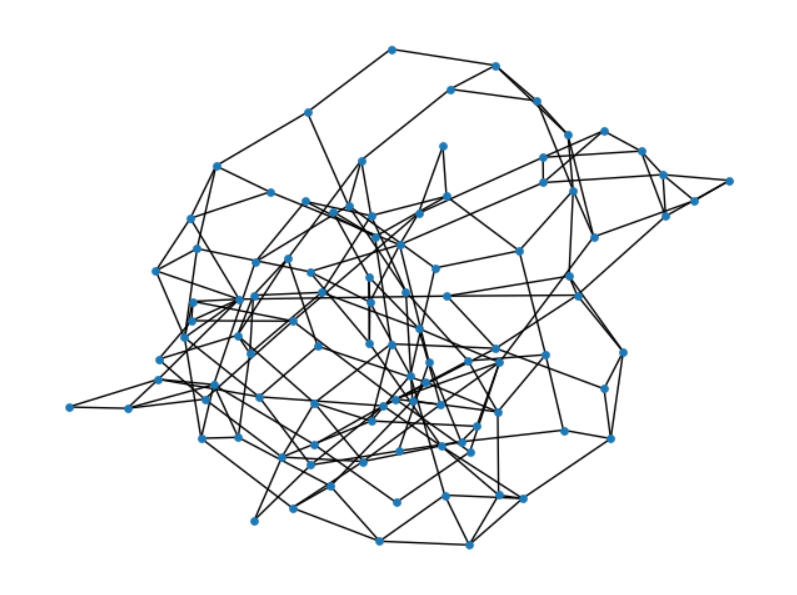
\includegraphics[width=\linewidth]{image/W_S_N100_K4_p0,3.png}
    \end{subfigure}
    \caption{Two example of Watts-Strogatz small world networks: on the left, it has 100 nodes, $K=2$ and $p=0.1$; on the right, it has 100 nodes, $K=4$ and $p=0.3$.}
    \label{W-S_example}
\end{figure}

The B-A and W-S algorithms produce more realistic networks respect to the E-R one, but both focus on their special feature: the B-A network fails to reproduce the high clustering of real network and the W-S one fails to reproduce the hubs  characteristic of scale-free networks.